\documentclass{article}
\usepackage[utf8]{inputenc}
\usepackage{amsmath}
\usepackage{graphicx}
%\usepackage{enumerate}
\usepackage{amsfonts}
\usepackage{natbib}
\usepackage{url} % not crucial - just used below for the URL 
\usepackage{cleveref}
\usepackage{float}
\usepackage[linesnumbered,ruled]{algorithm2e}
\usepackage{subfigure}
%\usepackage{lineno,hyperref} 
\usepackage{xcolor}

%\pdfminorversion=4
% NOTE: To produce blinded version, replace "0" with "1" below.
\newcommand{\blind}{0}
\let\oldref\ref
\renewcommand{\ref}[1]{(\oldref{#1})}
\DeclareMathOperator*{\argmin}{argmin}
\DeclareMathOperator*{\argmax}{argmax}


\newtheorem{prop}{Proposition}
\newtheorem{assumption}{Assumption}
\newtheorem{thm}{Theorem}
\newtheorem{proof}{Proof}


\title{Robust Boosting for Functional Regression}
%author{xmengju }
%\date{March 2021}

\begin{document}
\maketitle

\section{Introduction}
Nowadays, functional data has become more and mode widely available and has applications in a vast number of fields. Practitioners frequently observe data that can be described as functions defined on a domain (of time for instance). This kind of variables is inherently infinite-dimensional but are usually measured discretely.  

In the context of functional data analysis (FDA), a common problem is to estimate a regression model when the explanatory variable is functional. We assume that $(X_1, Y_1), ..., (X_n, Y_n)$ are independent and identically distributed realizations of the pair $(X, Y)$, where $Y\in \mathbb{R}$ is the response variable and $X \in L^2(\mathcal{I})$ is a square integrable function defined on an interval $\mathcal{I}$, and consider the multi-index model 
\begin{equation}\label{eq:1}
	Y = r(\langle X, \alpha_1 \rangle, ...,\langle X, \alpha_p \rangle ) + \epsilon,
\end{equation}
where $\langle X, \alpha_j \rangle = \int_{\mathcal{I}} X(t)\alpha_j(t)dt$, $\alpha_j \in L^2(\mathcal{I})$ are projection coefficients, $r: \mathbb{R}^p$ is an unknown smooth function, and $\epsilon$ is independent of $X$. 

 Previously, we found an approximation to $r$ in \ref{eq:1} using \texttt{TFBoost}, which yielded an estimator given by:
\begin{equation} 
\hat{r}_1(\langle X, \beta_{1,1} \rangle, ...,\langle X, \beta_{1,K}  \rangle) + ... + \hat{r}_M(\langle X, \beta_{M,1} \rangle, ...,\langle X, \beta_{M,K}  \rangle).
\end{equation}
The \texttt{TFBoost} algorithm used a ``functional multi-index trees" to compute each $r_j$, where each tree was constructed with $K$ projections ($\langle X, \beta_{j,1} \rangle, ...,\langle X, \beta_{j,K}  \rangle$) which we refer to as ``indices".  

In principle, \texttt{TFBoost} applies to data without  outliers, which are atypical observations  that deviate from the bulk of the data.  In practical situations, however,  measurements in the response and the functional predictor may either or both contain outlying values. Borrowing the terminology from \cite{rousseeuw1990unmasking} for linear regression, we refer to $(X_i, Y_i)$ as an ``leverage point"  if $X_i$ deviates from the majority of the data. This is only in regard to the outlyingness of $X$ and does not take the response $Y$ into consideration. If a leverage point $(X_i, Y_i)$ deviates greatly from the X-Y plane that  corresponds to the majority of the data, we call it a ``bad leverage point".  If we were to use the true model (the one that describes most data points) to predict $Y_i$, then a bad leverage point will have an extreme residual value.  On the other hand, if a leverage point  $(X_i, Y_i)$ is well represented by the true model, we call it a ``good leverage point".  A point $(X_i, Y_i)$ that is not a leverage point and does not follow the true model is called a ``vertical outlier". 

It is well-known atypical data points can seriously  affect the fit of the regression function. These points are $(X_i, Y_i)$ pairs that follow a model different from the  one that represents the majority of the data, including ``bad leverage points" and ``vertical outliers" depending on the outlyingness of $X_i$.  For functional predictors, the outliers in $X_i$ can exhibit  different properties: some present different shapes than the vast majority of the data and others have extreme values in some part of or across the domain.   The former are usually referred to as ``shape outliers" and the latter as ``magnitude outliers" \citep{hyndman2010rainbow, arribas2014shape, dai2020functional}.
 

Methods for functional regression in the presence of outliers have been developed in the past decade. Not many proposals exist and most are focused on linear models with vertical outliers. For the very few papers that considered bad leverage points, they either studied shape outliers or magnitude outliers, but not both. 


In what follows, we present a robust \texttt{TFBoost} algorithm for functional regression and assess its performance on data with different contaminations.    In the simulation study, we compare our estimator  with existing proposals on robust functional regression and functional additive regression estimators in a wide range of settings, which   cover cases without outliers and cases with bad leverage shape outliers,  bad leverage magnitude outliers, or vertical outliers. 
 

%can be viewed as infinite dimensional and has lead to 


%presents challenge to develop methods that takes into account of the functional nature of the  data. 


\section{Related work}
The impact of outliers has been extensively studied in the context of multivariate regression and numerous robust methods have been developed, especially for linear models.  In the functional context, this topic is less explored.  

Consider a general  model for functional regression
\begin{equation}\label{eq:general}
Y = 	F(X) + \epsilon, 
\end{equation}
where $X \in L^2 (\mathcal{I})$, $Y \in \mathbb{R}$, $\epsilon$ is independent form $X$, and the regression function  $F$: $L^2 (\mathcal{I}) \rightarrow \mathbb{R}$. Traditionally, one defines $F$ as  the conditional mean $E(Y|X)$ which is the minimizer of 
$$E( (Y - F(X) )^2).$$
When the training data contain outliers, the conditional mean is  easily affected and thus can produce misleading results. To deal with this problem, one can instead model the conditional median.  The task then becomes to estimate $F$ that minimizes 
$$E( |Y - F(X)|).$$

A few proposals on functional quantile regression 
include the estimation of conditional median as a particular case. \cite{cardot2005quantile} and  \cite{kato2012estimation} considered methods that connected the conditional quantile of the response with a linear function of the functional variable. \cite{ferraty2005conditional} and \cite{crambes2008robust}  modelled the conditional quantile in a nonparametric way,  extending the functional Nadaraya-Watson estimator introduced by \cite{ferraty2002functional}.  \cite{chen2012conditional} took an indirect approach by modelling and inverting the  conditional distribution function. More recently, methods to estimate the conditional quantile have been developed for functional local linear regression \citep{kaid2017functional,al2019functional}, functional single index regression \citep{sang2020functional}, support vector machines \citep{crambes2013support}, and partial functional regression \citep{qingguo2017quantile}.  

Some other proposals adopted outlier-resistant loss functions to construct M-type estimators. ......(unfinished......q)


\section{Methodology}
We address here the problem to estimate the regression function $F: X \rightarrow Y$, where the explanatory variable $X \in L^2(\mathcal{I})$ and the response $Y \in \mathbb{R}$. Define the target function 
$$F = \argmin_{G}L(Y, G(x)),$$
over joint distribution of $(X,Y)$ where $L$ is a pre-specified loss function, we estimate $F$ by adapting the robust gradient boosting procedure (\texttt{RRBoost}) proposed  by \cite{ju2021robust}. 

The generalization of \texttt{RRBoost} to functional data requires using functional regressors as the base learners. A convenient choice is the type B tree adopted by our previously proposed \texttt{TFBoost}. We recall the two stage estimating procedure of \texttt{RRBoost} below and use type B trees as base learners to approximate the negative gradients in both stages:
\begin{itemize}
\item Stage 1:compute an S-type boosting estimator with high robustness but possibly low efficiency;
\item Stage 2:compute an M-type boosting estimator initialized at the function and scale estimators obtained in Stage 1.	
\end{itemize}
We call the resulted estimator \texttt{RTFBoost} and outline the algorithm as follows: 

 \vspace{0.3cm}
\begin{algorithm}[H]
    \SetKwInOut{Input}{Input}
    \SetKwInOut{Output}{Output}
     \SetKwInOut{Initialize}{Initialize}
      \SetKwInOut{Stagea}{Stage 1}
     \SetKwInOut{Stageb}{Stage 2}
    \Input{A data set $(\mathbf{x}_i, y_i),  i \in \mathcal{I}_{\text{train}}$  \\
       The number of stage 1 iterations $T_1$   \\ 
       The number of stage 2 iterations $T_2$   \\ 
    The maximum depth of type B trees $d$ \\
    The number of random directions of type B trees $P$ \\
    Basis $\boldsymbol{\psi} = \{\psi_1, ..., \psi_d\}$ \\
    Shrinkage parameter $\nu$}
    \Initialize{ $\hat{F}_0(\mathbf{x})$}
     \Stagea{} 
    \hspace{1cm}   
    \For{$t = 1:T_1$}
     {
       \hspace{1cm}  $\hat{\sigma}_n (\hat{F}_{t-1}) =  \{\sigma: \frac{1}{| \mathcal{I}_{\text{train}}|}\sum_{i \in \mathcal{I}_{\text{train}}} \rho_0 \left( \frac{y_i - \hat{F}_{t-1}(x_i)}{\sigma}\right) = \kappa\}$ \\
	 \hspace{1cm}  $C_t =  \left[\sum_{i \in \mathcal{I}_{\text{train}}} \psi_0 \left(\frac{y_i - \hat{F}_{t-1}(x_i)}{\hat{\sigma}_n (\hat{F}_{t-1} )}\right) \left(\frac{y_i - \hat{F}_{t-1}(x_i)}{\hat{\sigma}_n (\hat{F}_{t-1} )}\right)\right]^{-1}$ \\
       \hspace{1cm}   $g_{t,\ell} = -C_t\psi_0 \left(\frac{y_{\ell}- \hat{F}_{t-1}(x_{\ell})} {\hat{\sigma}_n (\hat{F}_{t-1})} \right)$  \\
      \hspace{1cm}  Sample $\mathcal{P} = \{\mathbf{p}_1,..., \mathbf{p}_P\}$ \\ 
        \hspace{1cm}  $h_t = \argmin_{h \in \mathcal{H}}  \sum_{i \in |\mathcal{I}_{\text{train}}|}  \left(g_{t,i} + h\left( \mathbf{p}_1^T\langle x_i \boldsymbol{\psi} \rangle, ..., \mathbf{p}_P^T\langle x_i \boldsymbol{\psi} \rangle \right) \right)^2$ \\
       \hspace{1cm}   $\alpha_t = \argmin_{\alpha} \hat{\sigma}\left(\hat{F}_{t-1} + \alpha h_t\right)$ \\
       \hspace{1cm}   $\hat{F}_{t}(x) = \hat{F}_{t-1}(x) +  \alpha_t h_t(x)$  \\
        }
      \hspace{1cm}  $\hat{\sigma} =  \hat{\sigma}_n(\hat{F}_{T_1})$ \\
     \Stageb{}
     \hspace{1cm}
     \For{ $t = 1:T_2$}
     {
            \hspace{1cm} $g_{t,i} = - \frac{1}{\hat{\sigma}_n }
	    \psi_1 \left(\frac{y_{i}  - \hat{F}_{T_1 + t-1}(\mathbf{x}_{i})}{\hat{\sigma}_n} \right)$ \\
	        \hspace{1cm}  Sample $\mathcal{P} = \{\mathbf{p}_1,..., \mathbf{p}_P\}$ \\ 
                \hspace{1cm}  $h_t = \argmin_{h \in \mathcal{H}}  \sum_{i \in |\mathcal{I}_{\text{train}}|}  \left(g_{t,i} + h\left( \mathbf{p}_1^T\langle x_i \boldsymbol{\psi} \rangle, ..., \mathbf{p}_P^T\langle x_i \boldsymbol{\psi} \rangle \right) \right)^2$ \\
                  \hspace{1cm}  $\alpha_t = \argmin_{\alpha} \sum_{i \in \mathcal{I}_{\text{train}}} \rho_1 \left( \frac{y_i  - \hat{F}_{T_1 + t-1}(x_i)  - \alpha h_t\left( x_i \right)}{\hat{\sigma}} \right)$ \\
            \hspace{1cm} $\hat{F}_{T_1 + t}(x) = \hat{F}_{T_1 + t-1}(x) +   \alpha_t h_t(x)$ 
        }
      \Output{$\hat{F}_{T_1 + T_2}(x)$} 
          \caption{RTFBoost algorithm}
            \label{code-rrboost}
\end{algorithm}

\subsection{Early stopping}
Same as for \texttt{RRBoost}, we use an early stopping rule to determine $T_1$ and $T_2$ in Algorithm \ref{code-rrboost} in order to mitigate overfitting. We monitor the validation loss: 
$$L_{1,\text{val}}(t) = \hat{\sigma}_{\text{val}}(\hat{F}_t),$$
for stage 1 where $\hat{\sigma}_{\text{val}}$ satisfies 
 $$\frac{1}{| \mathcal{I}_{\text{val}}|}\sum_{i \in \mathcal{I}_{\text{val}}} \rho_0 \left( \frac{y_i - \hat{F}_{t-1}(x_i)}{\hat{\sigma}_{\text{val}}}\right) = \kappa,$$
 and
$$L_{2,\text{val}}(t) = \sum_{i\in \mathcal{I}_{\text{val}}} \rho_1 \left( \frac{y_i  - \hat{F}_{T_1 + t}(x_i)}{\hat{\sigma}}\right)$$
for stage 2 where 
$\hat{\sigma} =  \hat{\sigma}_n(\hat{F}_{T_1})$. 

We let $T_{1,\text{max}}$  and $T_{2,\text{max}}$ be the maximum number of iterations allowed in each stage. The early stopping times for stage 1 and stage 2 are defined as 
$$T_1 = \argmin_{t=1,..., T_{1,\text{max}}} L_{1,\text{val}}(t)$$
and $$T_2 = \argmin_{t=1,..., T_{2,\text{max}}} L_{2,\text{val}}(t)$$
respectively. 

\subsection{Initialization}
\label{sec:init}
Since the loss functions involved in \texttt{RTFBoost} are typically non-convex, a reliable initialization step is required to avoid reaching a local optima with a large objective value.  
We suggest using a type B tree computed with the L1 loss, which we call ``multi-index LAD tree".  This generalizes \texttt{LADTree} recommended for \texttt{RRBoost} from multivariate variables to a functional variable. 

To fit a  multi-index  LAD tree, we first sample $P$ random directions ${\mathbf{p}_1,..., \mathbf{p}_P}$ that satisfy 
$\lVert\mathbf{p}_j\rVert = 1$  and $p_{j,1}>0$. Given a basis  $\boldsymbol{\psi} = \{\psi_1, ..., \psi_d\}$, we calculate the candidate indices 
$\{\mathbf{p}_1^T\langle x_i, \boldsymbol{\psi}\rangle,..., \mathbf{p}_P^T\langle x_i, \boldsymbol{\psi}\rangle \}$. At each node, a multi-idnex LAD tree finds the split that minimizes the average absolute value of the residuals in a step-wise manner. Specifically, let $i \in \mathcal{I}_o$ be all the observations at a node $o$ and $R_1(j,s) = \{i| \mathbf{p}_j^T \langle x_i, \boldsymbol{\psi} \rangle \leq s\}$ and $R_2(j,s) = \{i| \mathbf{p}_j^T \langle x_i, \boldsymbol{\psi} \rangle > s\}$  be the left and right regions of the split made on the $j$-th index, we search for the split by solving
$$\min_{j\in \{1,...,P\}} \left \{\min_{s} \left(\min_{z_1} \sum_{i \in \{\mathcal{I}_o \cap R_1(j, s)\}} |y_i - z_1| + \sum_{i \in \{\mathcal{I}_o \cap R_2(j, s)\}}|y_i - z_2| \right) \right \}. $$
This procedure is repeated until the tree reaches the maximum depth ($d_{\text{init}}$) or minimum number of observations per node ($m_{\text{init}}$). 

To select the parameters ($d_{\text{init}}$ and $m_{\text{init}}$) of the initial tree, we first fit \texttt{RTFBoost} using the median of the responses as the initial fit: $$\hat{F}_0(x) = \text{median}( \{y_i| i \in \mathcal{I}_{\text{train}}\}),$$
and flagged potential outliers ($\mathcal{I}_f$) as those with residuals deviating from their median by more than 3 times their MAD. Then we fit \texttt{RTFBoost} with multi-index LAD tree for  each combination of ($d_{\text{init}}$, $m_{\text{init}}$) under consideration,  and chose the one that performs the best on the validation set, where  the performance is evaluated as the absolute deviation of residuals of non-flagged validation data points: 
$$\sum_{i \in \mathcal{I}_{\text{val}}/\mathcal{I}_{\text{f}}} \left|y_i - \hat{F}_{T_1 + T_2}(x_i) \right|.$$



\section{Simulation}
\subsection{Data generation}
\begin{itemize}
    \item We generated data sets $D = \{(x_i, y_i), i = 1,..., N\}$, consisting of a predictor $x_i\in\mathcal{L}_2$ and a scalar response $y_i$ that follow the model: 
 \begin{equation} \label{eq:gen}
y_i = r(x_i) + \rho \epsilon_i,
\end{equation}
where the errors $\epsilon_i$ are i.i.d, $r$ is the regression function,  and  $\rho > 0$ is a constant that controls the signal-to-noise ratio (SNR): 
$$\text{SNR} = \frac{\text{Var}(r(X))}{\text{Var}(\rho\epsilon)}.$$
\item To sample the functional predictors $x_i$, we considered the model:

\begin{equation} \label{eq:xmodel}
    x_i(t) = \mu(t) + \sum_{p=1}^4 \sqrt{\lambda_j}\xi_{ij}\phi_j(t),
\end{equation}
where $\mu(t) = 2\text{sin}(t\pi) \text{exp}(1-t)$, $\lambda_1 = 0.8, \lambda_2 = 0.3, \lambda_3 = 0.2$, and $\lambda_4 = 0.1$,  $\xi_{ij}\sim N(0,1) $,  and $\phi_j$ are the first four eigenfunctions of the ``Mattern'' covariance function $\gamma(s,t)$ with parameters $\rho = 3, \sigma = 1, \nu = 1/3$: 
 $$\gamma(s,t) = C\left(\frac{\sqrt{2\nu}|s-t|}{\rho}\right), \ C(u) = \frac{\sigma^2 2^{1-\nu}}{\Gamma(\nu)} u^{\nu} K_{\nu}(u),$$
  where $\Gamma(.)$ is the Gamma function and $K_{\nu}$ is the modified Bessel function of the second kind. For each subject $i$, we evaluate $x_i$ on a dense and regular grid $t_1,..., t_{100}$ equally spaced in $\mathcal{I} = [0,1]$. 
\item We considered five regression functions:
\begin{itemize}

\item[- ]  $r_1(X) =  \int_{\mathcal{I}} \left (\text{sin} \left(\frac{3}{2} \pi t \right) +  \text{sin} \left(\frac{1}{2} \pi t \right)\right)X(t)dt,$
\item[- ]  $r_2(X) = (\xi_1 + \xi_2)^{1/3},$ where  $\xi_1 = \int_{\mathcal{I}} (X(t) - \mu(t))\psi_1(t) dt$ and $\xi_2 = \int_{\mathcal{I}} (X(t) - \mu(t))\psi_2(t) dt$ are projections onto the first two FPCs ($\psi_1$ and $\psi_2$) of $X$ with mean $\mu(t) = E(X(t))$, 
\item[- ]  $r_3(X) = 5\text{exp}\left (- \frac{1}{2}\left| \int_{\mathcal{I}} x(t)\log(|x(t)|)dt \right| \right),$
\item[- ] 
$r_4(X) = 5\text{sigmoid}\left(\int_{\mathcal{I}}X(t)^2 \text{sin}(2\pi t) dt \right),$ where  $\text{sigmoid}(u) = 1/(1+ \text{exp}(-u))$, and
\item[- ] 
$r_5(X) = 5 \left( \sqrt{\left|\int_{\mathcal{I}_1} \text{cos}(2\pi t^2) X(t) dt \right|} + \sqrt{\left|\int_{\mathcal{I}_2} \text{sin}(X(t)) dt \right|} \right), $ where  $\mathcal{I}_1 = [0,0.5]$ and $\mathcal{I}_2 = (0.5,1]$. 
\end{itemize}

\item For clean data ($C_0$), we generated $\epsilon_i$ in \ref{eq:gen} from $N(0,1)$ and selected $\rho$ that corresponds to SNR = 5. 

For contaminated data, we sampled 10\% training samples as outliers and let the set of their indices be $\mathcal{O}$. The outliers belong to  one of the five types introduced below. For $j \in \mathcal{O}$, 
$$y_i = r(x_i) + \eta_i$$
\begin{itemize}
    \item[- ] $C_1$: \textit{Shape outliers}
    
    \vspace{1ex}
    In \ref{eq:xmodel},   $\xi_{j,2} \sim N(2, 0.25)$, $\mu(t) = 1 + 2\ \text{cos}(2t\pi)$, and the other parameters are the same as the model for clean data,
    \vspace{1ex}
    \item[- ] $C_2$: \textit{Magnitude outliers (curve-type)}     \vspace{1ex}
    
    $x_{j} = 2 \tilde{x}_{j} + 5$, where $\tilde{x}_j$ follows the model for clean data,
       \vspace{1ex}
    \item[- ] $C_3$: \textit{Magnitude outliers (point-type)}
    
       \vspace{1ex}
   Randomly sample 10  points form $t_1,..., t_{100}$ and denote them as $t_{j,o_1},..., t_{j,o_{10}}$. For $k = 1,..., 10$,   
    $$x_{j}(t_{j,o_k}) = \tilde{x}_j(t_{j,o_k}) + \eta_{j,o_k},$$ where $\eta_{j,o_k} \sim 0.5 N(10, 0.25) + 0.5 N(-10, 0.25)$, where
 $\tilde{x}_j$ follows the model for clean data,
    \vspace{1ex}
    \item[- ] $C_4$: \textit{Magnitude outliers (interval-type)}

    
       \vspace{1ex}
     Randomly sample one interval from intervals $[t_1,...,t_{10}]$, ...,$[t_{91},...,t_{100}]$,   and denote the interval as $t_{j,o},..., t_{j,o+9}$
     
     For $k = 0,..., 9$,   
    $$x_{j}(t_{j,o + k}) = \tilde{x}_j(t_{j,o + k}) + \eta_{j,o+k},$$ where $\eta_{j,o + k} \sim  N(10, 0.25)$, and 
 $\tilde{x}_j$ follows the model for clean data
    \vspace{1ex}
 
    \item[- ] $C_5$: \textit{vertical outliers} 
       \vspace{1ex}
   $$ x_j = \tilde{x}_j,$$
   where $\tilde{x}_j$ follows the model for clean data. 
\end{itemize}
For contaminated settings $C_1$,..., $C_5$, we generate $\eta_i$ from $$ 0.5N(30,0.25) + 0.5N(-30,0.25)$$
\end{itemize}


%\subsection{Visualize the outliers}


\subsection{Visualization of the outliers}

\begin{figure}[H]
    \centering
    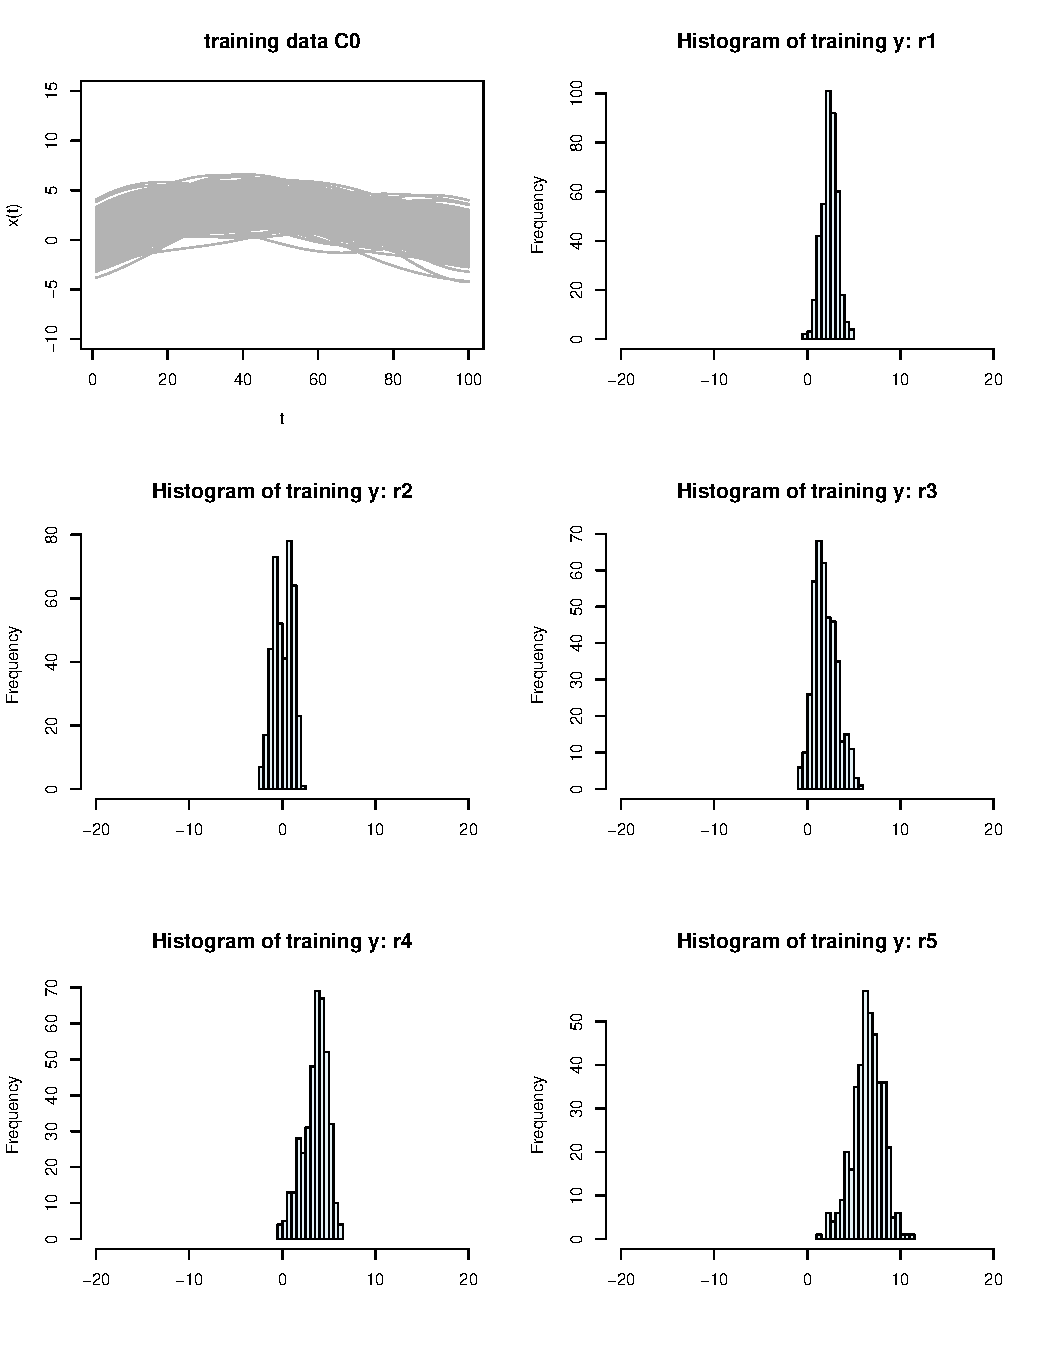
\includegraphics[scale = 0.7, page = 1]{visualize_outliers.pdf}
\end{figure}

\begin{figure}[H]
    \centering
    \includegraphics[scale = 0.7, page = 2]{visualize_outliers.pdf}
\end{figure}


\begin{figure}[H]
    \centering
    \includegraphics[scale = 0.7, page = 3]{visualize_outliers.pdf}
\end{figure}


\begin{figure}[H]
    \centering
    \includegraphics[scale = 0.7, page = 4]{visualize_outliers.pdf}
\end{figure}


\begin{figure}[H]
    \centering
    \includegraphics[scale = 0.7, page = 5]{visualize_outliers.pdf}
\end{figure}



\subsection{Model comparison}
For each setting, we used 100 independently generated datasets and compared the performance of the following methods: 

\begin{itemize}
 \setlength\itemsep{0.1em}
\item \texttt{FPPR}: functional projection pursuit regression \citep{ferraty2013functional},
\item \texttt{FGAM}: functional generalized additive models \citep{mclean2014functional}, 
\item \texttt{MFLM}: Sieve M-estimator for a semi-functional linear model \citep{huang2015sieve},
\item \texttt{RFSIR}: robust functional sliced inverse regression \citep{wang2017robust}
\item \texttt{RFPLM}: robust estimation for semi-functional linear regression models \citep{boente2020robust},
\item  \texttt{TFBoost(L2)}:  tree-based functional boosting with L2 loss,
\item  \texttt{TFBoost(LAD)}:  tree-based functional boosting with LAD loss,
\item  \texttt{TFBoost(RR)}:  proposed robust  tree-based functional boosting. 
\end{itemize}

\subsection{Implementation details}

\begin{itemize}
	\item For \texttt{FPPR}, we implemented the method based on the code to fit a functional single index model shared by  the authors of \cite{ferraty2013functional}.  We used cubic B-spline with 7 functions (3 evenly spaced interior knots) as the basis and selected the number of additive components between 1 to 15 to minimize the validation  robust  MSPE, which is defined as
	$$\text{median}( \{y_i - \hat{F}(x_i)\}|i \in \mathcal{I}_{\text{val}})^2 + \hat{\sigma}_M(  \{y_i - \hat{F}(x_i)\}|i \in \mathcal{I}_{\text{val}}),$$
	where $\hat{\sigma}_M$ is the M-scale estimator with 0.5 breakdown point and 95\% asymptotic efficiency at the normal model. 
	\item For \texttt{FGAM},  we adopted the implementation in \texttt{refund} package. We set basis to be bivariate cubic B-splines of dimension 15 by 15 and used REML to select penalization parameter. 
	\item For \texttt{MFLM} and \texttt{RFPLM}, we adopted the implementation available from \\ https://github.com/msalibian/RobustFPLM. We considered cubic B-spline basis of dimension 4 to 7 with evenly spaced interior knots, and selected the dimension that minimized the BIC. 
	\item For \texttt{RFSIR}, we used the code shared by the author of \cite{wang2017robust}. We selected the number of leading functional principal components from 1 to 10 to minimize the validation  robust  MSPE. 
	\item For \texttt{TFBoost(L2)},  \texttt{TFBoost(LAD)}, and  \texttt{RTFBoost}, we used type B trees as base learners. With each training data, we selected the maximum depth of type B tree from 1 to 4 that achieves the lowest validation robust MSPE. To initialize \texttt{RTFBoost}, we considered multi-index LADTree with  maximum depth equal to 1, 2, and 3, and the minimum number of observations per node equal to 10, 20, and 30, and selected their values following the procedure introduced in \Cref{sec:init}. 
\end{itemize}



\subsection{Simulation results}
Summary statistics of test MSPEs, displayed in the form of mean (sd). 
\texttt{TFBoost(RR.5)} and \texttt{TFBoost(RR.2)} were initialized with the median of training responses
% latex table generated in R 4.0.5 by xtable 1.8-4 package
% Wed Aug  4 02:25:06 2021
\renewcommand{\arraystretch}{1.5}
\addtolength{\tabcolsep}{-3pt} 

\begin{table}[H]
\centering
\footnotesize
\begin{tabular}{rllllll}
  \hline
 & $C_0$ & $C_1$ & $C_2$ & $C_3$ & $C_4$ & $C_5$ \\ 
  \hline
TFBoost(L2) & 0.146 (0.005) & 0.604 (0.304) & 0.878 (0.275) & 0.991 (0.317) & 1.163 (0.333) & 1.294 (0.806) \\ 
  TFBoost(LAD) & 0.151 (0.009) & 0.174 (0.061) & 0.204 (0.097) & 0.147 (0.014) & 0.214 (0.146) & 0.154 (0.012) \\ 
  TFBoost(LAD-M) & 0.148 (0.009) & 0.166 (0.029) & 0.177 (0.046) & 0.141 (0.013) & 0.187 (0.073) & 0.149 (0.010) \\ 
  TFBoost(RR.5) & 0.166 (0.044) & 0.160 (0.020) & 0.190 (0.079) & 0.144 (0.012) & 0.166 (0.042) & 0.150 (0.011) \\ 
  TFBoost(RR.2) & 0.150 (0.010) & 0.150 (0.009) & \textbf{0.159} (0.013) & 0.136 (0.005) & 0.146 (0.007) & 0.150 (0.013) \\ 
  FPPR & 0.137 (0.006) & 3.378 (3.725) & 1.787 (2.510) & 6.025 (4.312) & 9.691 (6.253) & 2.759 (2.671) \\ 
  FGAM & \textbf{0.130} (0.005) & 1.751 (2.464) & 2.732 (3.324) & 62.725 (182.870) & 6.073 (15.833) & 0.848 (0.456) \\ 
  RFPLM & 0.131 (0.006) & \textbf{0.131} (0.006) & \textbf{0.131} (0.006) & \textbf{0.120} (0.001) & \textbf{0.130} (0.002) & \textbf{0.131} (0.006) \\ 
  MFLM & \textbf{0.130} (0.005) & \textbf{0.138} (0.009) & 0.181 (0.052) & \textbf{0.129} (0.016) & 0.168 (0.026) & \textbf{0.139} (0.011) \\ 
  RFSIR & 0.138 (0.007) & 0.465 (0.438) & 1.113 (0.932) & 0.130 (0.004) & \textbf{0.140} (0.006) & 1.207 (1.229) \\ 
   \hline
\end{tabular}
\caption{Summary statistics of test errors for data generated from $r_1$; displayed in the form of mean (sd).} 
\end{table}
% latex table generated in R 4.0.5 by xtable 1.8-4 package
% Wed Aug  4 02:25:26 2021
\begin{table}[H]
\centering
\footnotesize
\begin{tabular}{rllllll}
  \hline
 & $C_0$ & $C_1$ & $C_2$ & $C_3$ & $C_4$ & $C_5$ \\ 
  \hline
TFBoost(L2) & \textbf{0.183} (0.010) & 0.791 (0.393) & 1.031 (0.123) & 1.178 (0.285) & 1.485 (0.244) & 2.338 (1.533) \\ 
  TFBoost(LAD) & 0.188 (0.009) & 0.232 (0.148) & 0.245 (0.116) & 0.180 (0.010) & 0.268 (0.135) & 0.191 (0.017) \\ 
  TFBoost(LAD-M) & 0.187 (0.009) & 0.213 (0.092) & \textbf{0.212} (0.091) & 0.180 (0.012) & 0.263 (0.135) & \textbf{0.187} (0.015) \\ 
  TFBoost(RR.5) & 0.203 (0.039) & \textbf{0.192} (0.012) & 0.232 (0.056) & 0.189 (0.048) & \textbf{0.194} (0.016) & 0.207 (0.055) \\ 
  TFBoost(RR.2) & 0.189 (0.014) & \textbf{0.184} (0.011) & \textbf{0.187} (0.013) & \textbf{0.171} (0.007) & \textbf{0.181} (0.006) & \textbf{0.186} (0.011) \\ 
  FPPR & \textbf{0.182} (0.010) & 4.119 (3.694) & 3.156 (3.078) & 7.945 (6.784) & 9.384 (4.534) & 3.295 (2.602) \\ 
  FGAM & 0.226 (0.010) & 1.972 (2.451) & 2.941 (2.394) & 55.296 (163.996) & 6.197 (15.351) & 0.995 (0.475) \\ 
  RFPLM & 0.285 (0.012) & 0.283 (0.013) & 0.286 (0.013) & 0.274 (0.011) & 0.281 (0.014) & 0.286 (0.016) \\ 
  MFLM & 0.283 (0.011) & 0.358 (0.144) & 0.526 (0.197) & 0.567 (0.153) & 0.709 (0.056) & 0.477 (0.190) \\ 
  RFSIR & 0.184 (0.009) & 0.682 (0.636) & 1.647 (2.307) & \textbf{0.171} (0.005) & 0.199 (0.027) & 1.356 (1.319) \\ 
   \hline
\end{tabular}
\caption{Summary statistics of test errors for data generated from $r_2$; displayed in the form of mean (sd).} 
\end{table}
% latex table generated in R 4.0.5 by xtable 1.8-4 package
% Wed Aug  4 02:25:45 2021
\begin{table}[H]
\centering
\footnotesize
\begin{tabular}{rllllll}
  \hline
 & $C_0$ & $C_1$ & $C_2$ & $C_3$ & $C_4$ & $C_5$ \\ 
  \hline
TFBoost(L2) & \textbf{0.309} (0.013) & 0.983 (0.532) & 1.534 (0.325) & 1.668 (0.170) & 2.054 (0.250) & 2.414 (1.502) \\ 
  TFBoost(LAD) & 0.318 (0.018) & 0.400 (0.196) & 0.368 (0.091) & 0.300 (0.017) & 0.374 (0.100) & 0.326 (0.022) \\ 
  TFBoost(LAD-M) & 0.315 (0.016) & 0.355 (0.113) & \textbf{0.351} (0.089) & 0.296 (0.015) & 0.357 (0.092) & \textbf{0.321} (0.017) \\ 
  TFBoost(RR.5) & 0.443 (0.321) & \textbf{0.344} (0.064) & 0.420 (0.174) & 0.299 (0.014) & 0.375 (0.164) & 0.409 (0.207) \\ 
  TFBoost(RR.2) & 0.335 (0.069) & \textbf{0.320} (0.016) & \textbf{0.313} (0.021) & \textbf{0.290} (0.011) & \textbf{0.308} (0.012) & \textbf{0.315} (0.020) \\ 
  FPPR & \textbf{0.305} (0.019) & 3.352 (3.087) & 2.699 (3.097) & 6.614 (6.942) & 8.806 (4.622) & 2.996 (2.215) \\ 
  FGAM & 0.321 (0.017) & 2.006 (2.452) & 3.825 (3.861) & 52.164 (147.124) & 6.453 (15.311) & 1.107 (0.459) \\ 
  RFPLM & 0.380 (0.018) & 0.383 (0.017) & 0.380 (0.019) & 0.363 (0.014) & 0.386 (0.025) & 0.380 (0.021) \\ 
  MFLM & 0.377 (0.018) & 0.394 (0.021) & 0.475 (0.082) & 0.415 (0.030) & 2.596 (0.186) & 0.404 (0.024) \\ 
  RFSIR & 0.313 (0.018) & 2.423 (3.818) & 1.758 (2.426) & \textbf{0.292} (0.026) & \textbf{0.310} (0.016) & 1.455 (0.940) \\ 
   \hline
\end{tabular}
\caption{Summary statistics of test errors for data generated from $r_3$; displayed in the form of mean (sd).} 
\end{table}
% latex table generated in R 4.0.5 by xtable 1.8-4 package
% Wed Aug  4 02:26:03 2021
\begin{table}[H]
\centering
\footnotesize
\begin{tabular}{rllllll}
  \hline
 & $C_0$ & $C_1$ & $C_2$ & $C_3$ & $C_4$ & $C_5$ \\ 
  \hline
TFBoost(L2) & \textbf{0.323} (0.015) & 1.042 (0.583) & 1.650 (0.312) & 1.902 (0.326) & 2.147 (0.241) & 2.362 (1.188) \\ 
  TFBoost(LAD) & 0.332 (0.013) & 0.448 (0.181) & 0.403 (0.118) & 0.323 (0.022) & 0.504 (0.247) & 0.354 (0.041) \\ 
  TFBoost(LAD-M) & 0.332 (0.020) & 0.410 (0.169) & \textbf{0.368} (0.114) & \textbf{0.313} (0.016) & 0.470 (0.231) & \textbf{0.338} (0.036) \\ 
  TFBoost(RR.5) & 0.398 (0.191) & \textbf{0.402} (0.158) & 0.388 (0.137) & 0.347 (0.112) & 0.359 (0.126) & 0.363 (0.116) \\ 
  TFBoost(RR.2) & \textbf{0.331} (0.018) & \textbf{0.334} (0.018) & \textbf{0.334} (0.022) & \textbf{0.305} (0.015) & \textbf{0.326} (0.015) & \textbf{0.332} (0.022) \\ 
  FPPR & 0.364 (0.030) & 3.899 (3.073) & 3.696 (3.489) & 7.516 (5.231) & 10.841 (5.110) & 4.360 (2.674) \\ 
  FGAM & 0.409 (0.020) & 2.031 (2.307) & 3.775 (3.793) & 44.480 (120.133) & 6.741 (16.325) & 1.511 (0.452) \\ 
  RFPLM & 0.542 (0.034) & 0.544 (0.037) & 0.546 (0.043) & 0.525 (0.028) & 0.552 (0.028) & 0.546 (0.040) \\ 
  MFLM & 0.537 (0.032) & 0.610 (0.149) & 0.709 (0.168) & 0.825 (0.141) & 1.024 (0.106) & 0.764 (0.165) \\ 
  RFSIR & 0.340 (0.018) & 1.447 (1.648) & 3.148 (3.282) & 0.328 (0.018) & \textbf{0.352} (0.019) & 1.803 (0.843) \\ 
   \hline
\end{tabular}
\caption{Summary statistics of test errors for data generated from $r_4$; displayed in the form of mean (sd).} 
\end{table}
% latex table generated in R 4.0.5 by xtable 1.8-4 package
% Wed Aug  4 02:26:19 2021
\begin{table}[H]
\centering
\footnotesize
\begin{tabular}{rllllll}
  \hline
 & $C_0$ & $C_1$ & $C_2$ & $C_3$ & $C_4$ & $C_5$ \\ 
  \hline
TFBoost(L2) & \textbf{0.585} (0.033) & 1.297 (0.608) & 2.375 (0.595) & 2.350 (0.279) & 2.654 (0.265) & 2.918 (1.232) \\ 
  TFBoost(LAD) & 0.618 (0.032) & 0.685 (0.133) & 0.743 (0.084) & 0.597 (0.043) & 0.776 (0.203) & 0.656 (0.052) \\ 
  TFBoost(LAD-M) & 0.607 (0.035) & 0.658 (0.127) & \textbf{0.690} (0.104) & \textbf{0.571} (0.023) & 0.762 (0.196) & \textbf{0.616} (0.045) \\ 
  TFBoost(RR.5) & 0.734 (0.220) & \textbf{0.645} (0.059) & 0.735 (0.172) & 0.631 (0.097) & 0.687 (0.155) & 0.670 (0.060) \\ 
  TFBoost(RR.2) & 0.637 (0.043) & \textbf{0.602} (0.043) & \textbf{0.624} (0.032) & \textbf{0.567} (0.031) & \textbf{0.610} (0.033) & \textbf{0.608} (0.036) \\ 
  FPPR & 0.607 (0.062) & 4.380 (3.473) & 3.035 (3.747) & 6.109 (4.047) & 9.940 (3.798) & 4.196 (3.162) \\ 
  FGAM & \textbf{0.606} (0.041) & 2.278 (2.458) & 5.049 (5.805) & 43.774 (117.297) & 7.048 (13.854) & 1.857 (0.516) \\ 
  RFPLM & 0.896 (0.048) & 0.871 (0.053) & 0.892 (0.052) & 0.849 (0.040) & 0.896 (0.046) & 0.888 (0.053) \\ 
  MFLM & 0.883 (0.040) & 0.891 (0.045) & 1.034 (0.166) & 0.944 (0.071) & 2.009 (0.817) & 0.932 (0.071) \\ 
  RFSIR & 0.680 (0.056) & 2.423 (2.383) & 2.211 (1.382) & 0.628 (0.038) & \textbf{0.638} (0.049) & 1.979 (0.973) \\ 
   \hline
\end{tabular}
\caption{Summary statistics of test errors for data generated from $r_5$; displayed in the form of mean (sd).} 
\end{table}


Summary statistics of test MSPEs, displayed in the form of mean (sd). 
\texttt{TFBoost(RR.5)} and \texttt{TFBoost(RR.2)} were initialized with the \texttt{LADTrees} with the maximum depth chosen from $\{0,1,2,3\}$ and the minimum number of observations per node chosen from 
$\{10,20,30\}$. 
% latex table generated in R 4.0.5 by xtable 1.8-4 package
% Mon Aug  2 23:50:53 2021
\renewcommand{\arraystretch}{1.5}
\addtolength{\tabcolsep}{-3pt}    
\begin{table}[H]
\footnotesize
\centering
\begin{tabular}{rllllll}
  \hline
 & $C_0$ & $C_1$ & $C_2$ & $C_3$ & $C_4$ & $C_5$ \\ 
  \hline
TFBoost(L2) & 0.146 (0.005) & 0.604 (0.304) & 0.878 (0.275) & 0.991 (0.317) & 1.163 (0.333) & 1.294 (0.806) \\ 
  TFBoost(LAD) & 0.150 (0.009) & 0.197 (0.110) & 0.194 (0.070) & 0.147 (0.014) & 0.250 (0.195) & 0.153 (0.010) \\ 
  TFBoostLAD-M) & 0.148 (0.009) & 0.285 (0.173) & 0.222 (0.069) & 0.172 (0.026) & 0.486 (0.372) & 0.152 (0.011) \\ 
  TFBoost(RR) & 0.150 (0.010) & 0.804 (1.765) & 0.284 (0.391) & 0.268 (0.317) & 1.306 (2.452) & 0.150 (0.013) \\ 
  FPPR & 0.137 (0.006) & 3.378 (3.725) & 1.787 (2.510) & 6.025 (4.312) & 9.691 (6.253) & 2.759 (2.671) \\ 
  FGAM & \textbf{0.130} (0.005) & 1.751 (2.464) & 2.732 (3.324) & 62.725 (182.870) & 6.073 (15.833) & 0.848 (0.456) \\ 
  RFPLM & 0.131 (0.006) & \textbf{0.131} (0.006) & \textbf{0.131} (0.006) & \textbf{0.120} (0.001) & \textbf{0.130} (0.002) & \textbf{0.131} (0.006) \\ 
  MFLM & \textbf{0.130} (0.005) & \textbf{0.138} (0.009) & \textbf{0.181} (0.052) & \textbf{0.129} (0.016) & 0.168 (0.026) & \textbf{0.139} (0.011) \\ 
  RFSIR & 0.138 (0.007) & 0.465 (0.438) & 1.113 (0.932) & 0.130 (0.004) & \textbf{0.140} (0.006) & 1.207 (1.229) \\ 
   \hline
\end{tabular}
\caption{Summary statistics of test errors for data generated from $r_1$; displayed in the form of mean (sd).} 
\end{table}
% latex table generated in R 4.0.5 by xtable 1.8-4 package
% Mon Aug  2 23:51:08 2021
\begin{table}[H]
\footnotesize
\centering
\begin{tabular}{rllllll}
  \hline
 & $C_0$ & $C_1$ & $C_2$ & $C_3$ & $C_4$ & $C_5$ \\ 
  \hline
TFBoost(L2) & \textbf{0.183} (0.010) & 0.703 (0.369) & 1.013 (0.155) & 1.178 (0.285) & 1.468 (0.270) & 2.338 (1.533) \\ 
  TFBoost(LAD) & 0.186 (0.008) & \textbf{0.258} (0.167) & \textbf{0.251} (0.122) & 0.178 (0.008) & \textbf{0.254} (0.117) & \textbf{0.190} (0.014) \\ 
  TFBoostLAD-M) & 0.190 (0.008) & 0.333 (0.185) & 0.319 (0.266) & 0.224 (0.044) & 0.498 (0.251) & 0.195 (0.016) \\ 
  TFBoost(RR) & 0.192 (0.016) & \textbf{0.186} (0.011) & 0.848 (2.711) & \textbf{0.175} (0.013) & 0.404 (0.626) & \textbf{0.190} (0.017) \\ 
  FPPR & \textbf{0.182} (0.010) & 4.119 (3.694) & 3.156 (3.078) & 7.945 (6.784) & 9.384 (4.534) & 3.295 (2.602) \\ 
  FGAM & 0.226 (0.010) & 1.972 (2.451) & 2.941 (2.394) & 55.296 (163.996) & 6.197 (15.351) & 0.995 (0.475) \\ 
  RFPLM & 0.285 (0.012) & 0.283 (0.013) & \textbf{0.286} (0.013) & 0.274 (0.011) & 0.281 (0.014) & 0.286 (0.016) \\ 
  MFLM & 0.283 (0.011) & 0.358 (0.144) & 0.526 (0.197) & 0.567 (0.153) & 0.709 (0.056) & 0.477 (0.190) \\ 
  RFSIR & 0.184 (0.009) & 0.682 (0.636) & 1.647 (2.307) & \textbf{0.171} (0.005) & \textbf{0.199} (0.027) & 1.356 (1.319) \\ 
   \hline
\end{tabular}
\caption{Summary statistics of test errors for data generated from $r_2$; displayed in the form of mean (sd).} 
\end{table}
% latex table generated in R 4.0.5 by xtable 1.8-4 package
% Mon Aug  2 23:51:22 2021
\begin{table}[H]
\footnotesize
\centering
\begin{tabular}{rllllll}
  \hline
 & $C_0$ & $C_1$ & $C_2$ & $C_3$ & $C_4$ & $C_5$ \\ 
  \hline
TFBoost(L2) & \textbf{0.309} (0.013) & 0.956 (0.546) & 1.499 (0.360) & 1.668 (0.170) & 2.042 (0.248) & 2.414 (1.502) \\ 
  TFBoost(LAD) & 0.316 (0.016) & \textbf{0.391} (0.131) & \textbf{0.377} (0.090) & 0.301 (0.017) & 0.423 (0.203) & \textbf{0.324} (0.024) \\ 
  TFBoostLAD-M) & 0.317 (0.015) & 0.450 (0.130) & 0.395 (0.109) & 0.337 (0.043) & 0.641 (0.405) & 0.329 (0.023) \\ 
  TFBoost(RR) & 0.324 (0.032) & 0.710 (1.743) & 0.469 (0.477) & \textbf{0.290} (0.011) & \textbf{0.313} (0.021) & \textbf{0.315} (0.020) \\ 
  FPPR & \textbf{0.305} (0.019) & 3.352 (3.087) & 2.699 (3.097) & 6.614 (6.942) & 8.806 (4.622) & 2.996 (2.215) \\ 
  FGAM & 0.321 (0.017) & 2.006 (2.452) & 3.825 (3.861) & 52.164 (147.124) & 6.453 (15.311) & 1.107 (0.459) \\ 
  RFPLM & 0.380 (0.018) & \textbf{0.383} (0.017) & \textbf{0.380} (0.019) & 0.363 (0.014) & 0.386 (0.025) & 0.380 (0.021) \\ 
  MFLM & 0.377 (0.018) & 0.394 (0.021) & 0.475 (0.082) & 0.415 (0.030) & 2.596 (0.186) & 0.404 (0.024) \\ 
  RFSIR & 0.313 (0.018) & 2.423 (3.818) & 1.758 (2.426) & \textbf{0.292} (0.026) & \textbf{0.310} (0.016) & 1.455 (0.940) \\ 
   \hline
\end{tabular}
\caption{Summary statistics of test errors for data generated from $r_3$; displayed in the form of mean (sd).} 
\end{table}
% latex table generated in R 4.0.5 by xtable 1.8-4 package
% Mon Aug  2 23:51:36 2021
\begin{table}[H]
\footnotesize
\centering
\begin{tabular}{rllllll}
  \hline
 & $C_0$ & $C_1$ & $C_2$ & $C_3$ & $C_4$ & $C_5$ \\ 
  \hline
TFBoost(L2) & \textbf{0.323} (0.015) & 0.884 (0.472) & 1.596 (0.382) & 1.941 (0.344) & 2.073 (0.247) & 2.514 (1.598) \\ 
  TFBoost(LAD) & 0.335 (0.014) & \textbf{0.401} (0.140) & \textbf{0.392} (0.070) & \textbf{0.317} (0.017) & 0.565 (0.328) & 0.351 (0.039) \\ 
  TFBoostLAD-M) & \textbf{0.333} (0.020) & \textbf{0.470} (0.167) & \textbf{0.432} (0.128) & 0.343 (0.026) & 0.728 (0.382) & \textbf{0.343} (0.034) \\ 
  TFBoost(RR) & 0.335 (0.025) & 0.879 (2.194) & 0.468 (0.417) & \textbf{0.313} (0.035) & 1.252 (2.085) & \textbf{0.340} (0.034) \\ 
  FPPR & 0.364 (0.030) & 3.899 (3.073) & 3.696 (3.489) & 7.516 (5.231) & 10.841 (5.110) & 4.360 (2.674) \\ 
  FGAM & 0.409 (0.020) & 2.031 (2.307) & 3.775 (3.793) & 44.480 (120.133) & 6.741 (16.325) & 1.511 (0.452) \\ 
  RFPLM & 0.542 (0.034) & 0.544 (0.037) & 0.546 (0.043) & 0.525 (0.028) & \textbf{0.552} (0.028) & 0.546 (0.040) \\ 
  MFLM & 0.537 (0.032) & 0.610 (0.149) & 0.709 (0.168) & 0.825 (0.141) & 1.024 (0.106) & 0.764 (0.165) \\ 
  RFSIR & 0.340 (0.018) & 1.447 (1.648) & 3.148 (3.282) & 0.328 (0.018) & \textbf{0.352} (0.019) & 1.803 (0.843) \\ 
   \hline
\end{tabular}
\caption{Summary statistics of test errors for data generated from $r_4$; displayed in the form of mean (sd).} 
\end{table}
% latex table generated in R 4.0.5 by xtable 1.8-4 package
% Mon Aug  2 23:51:52 2021
\begin{table}[H]
\footnotesize
\centering
\begin{tabular}{rllllll}
  \hline
 & $C_0$ & $C_1$ & $C_2$ & $C_3$ & $C_4$ & $C_5$ \\ 
  \hline
TFBoost(L2) & \textbf{0.586} (0.034) & 1.087 (0.429) & 2.274 (0.690) & 2.369 (0.300) & 2.625 (0.289) & 3.078 (1.355) \\ 
  TFBoost(LAD) & 0.617 (0.033) & \textbf{0.726} (0.216) & \textbf{0.705} (0.054) & 0.603 (0.031) & \textbf{0.698} (0.098) & 0.649 (0.054) \\ 
  TFBoostLAD-M) & 0.607 (0.035) & \textbf{0.743} (0.196) & \textbf{0.740} (0.145) & \textbf{0.583} (0.038) & 0.875 (0.228) & \textbf{0.619} (0.048) \\ 
  TFBoost(RR) & 0.643 (0.045) & 0.825 (0.990) & 1.107 (1.602) & \textbf{0.578} (0.048) & 1.176 (1.296) & \textbf{0.619} (0.049) \\ 
  FPPR & 0.607 (0.062) & 4.380 (3.473) & 3.035 (3.747) & 6.109 (4.047) & 9.940 (3.798) & 4.196 (3.162) \\ 
  FGAM & \textbf{0.606} (0.041) & 2.278 (2.458) & 5.049 (5.805) & 43.774 (117.297) & 7.048 (13.854) & 1.857 (0.516) \\ 
  RFPLM & 0.896 (0.048) & 0.871 (0.053) & 0.892 (0.052) & 0.849 (0.040) & 0.896 (0.046) & 0.888 (0.053) \\ 
  MFLM & 0.883 (0.040) & 0.891 (0.045) & 1.034 (0.166) & 0.944 (0.071) & 2.009 (0.817) & 0.932 (0.071) \\ 
  RFSIR & 0.680 (0.056) & 2.423 (2.383) & 2.211 (1.382) & 0.628 (0.038) & \textbf{0.638} (0.049) & 1.979 (0.973) \\ 
   \hline
\end{tabular}
\caption{Summary statistics of test errors for data generated from $r_5$; displayed in the form of mean (sd).} 
\end{table}

\bibliographystyle{apalike}
\bibliography{reference}
\end{document}
